\documentclass{article}

\usepackage[utf8]{inputenc}
\usepackage[ngerman]{babel}
\usepackage{amssymb}
\usepackage{amsmath}
\usepackage{graphics}
% Pseudocode
\usepackage{algorithm}
\usepackage[noend]{algpseudocode}
\usepackage{graphicx}

\setlength{\parindent}{0in}

\newcommand{\uebungsGruppe}{1}
\newcommand{\zettelNummer}{7}
\newcommand{\studierenderEins}{Eli Kogan-Wang (7251030)}
\newcommand{\studierenderZwei}{David Noah Stamm (7249709)}
\newcommand{\studierenderDrei}{Daniel Heins (7213874)}
\newcommand{\studierenderVier}{Tim Wolf (7269381)}

\newcounter{AufgabenCounter}
\setcounter{AufgabenCounter}{1}
\newcounter{TeilaufgabenCounter}
\newenvironment{aufgabe}{\section*{Aufgabe \theAufgabenCounter}\setcounter{TeilaufgabenCounter}{1}}{\stepcounter{AufgabenCounter}}
\newenvironment{teilaufgabe}{\paragraph*{\alph{TeilaufgabenCounter})}}{\stepcounter{TeilaufgabenCounter}}

\renewcommand{\to}{\textnormal{ to }}
\newcommand{\bigO}{\mathcal{O}}

\newcommand{\qed}{\hfill$\square$}

\begin{document}

\title{Datenstrukturen und Algorithmen \\ Heimübung \zettelNummer{}}
\author{\studierenderEins{} \\
  \studierenderZwei{} \\
  \studierenderDrei{} \\
  \studierenderVier{}}

\maketitle

% Aufgabe 1
\begin{aufgabe}
  Damit Prev(x) und Succ(x) in $\mathcal{O}(1)$ liegen, muss man eine zusätzliche Eigenschaft für alle Knoten im Baum definieren. \\
  Jeder Knoten x im Baum erhält zusätzlich eine Verweis auf die Adresse seines Nachfolgers und Vorgängers mit $N_x$ := die Adresse des Nachvolgers von x und $V_x$ := die Adresse des Vorgängers von x \\
  Damit dies Eigenschaft aufrecht erhalten wird müssen die Einfügen- und Löschenfunktion abgeändert werden.

  \begin{algorithm}[H]
    \caption{EinfügenNeu(T,z)}
    \begin{algorithmic}[1]
      \State $y \gets nil$
      \State $x \gets root[T]$
      \While{x $\neq$ nil}1
      \State $y \gets x$
      \If{$key[z] < key[x]$}
      \State $x \gets lc[x]$
      \Else
      \State $x \gets rc[x]$
      \EndIf
      \EndWhile
      \State $p[z] \gets y$
      \If{$y=nil$}
      \State $root[t] \gets z$
      \State $V[z] \gets nil$
      \State $N[z] \gets nil$
      \Else
      \If{$key[z] < key[y]$}
      \State $lc[y] \gets z$
      \State $N_{V_y} \gets z$
      \State $V_z \gets V_y$
      \State $V_y \gets z$
      \State $N_z \gets y$
      \Else
      \State $rc[y] \gets z$
      \State $V_{N_y} \gets z$
      \State $N_z \gets N_y$
      \State $N_y \gets z$
      \State $V_z \gets y$
      \EndIf
      \EndIf
    \end{algorithmic}
  \end{algorithm}

  \begin{algorithm}[H]
    \caption{LöschenNeu(T,z)}
    \begin{algorithmic}[1]
      \If{$lc[z] = nil\lor rc[z] = nil$}
      \State $y \gets z$
      \Else
      \State $y \gets N_z$
      \EndIf
      \If{$V_y \neq nil$}
      \State $N_{V_y} \gets N_z$
      \EndIf
      \If{$N_y \neq nil$}
      \State $V_{N_y} \gets V_z$
      \EndIf
      \If{$V_z \neq nil$}
      \State $N_{V_z} \gets N_z$
      \EndIf
      \If{$N_z \neq nil$}
      \State $V_{N_z} \gets V_z$
      \EndIf
      \If{$lc[y] \neq nil$}
      \State $x \gets lc[y]$
      \Else
      \State $x \gets rc[y]$
      \EndIf
      \If{$x \neq nil$}
      \State $p[x] \gets p[y]$
      \EndIf
      \If{$p[y] = nil$}
      \State $root[T] \gets x$
      \Else
      \If{$y = lc[p[y]]$}
      \State $lc[p[y]] \gets x$
      \Else
      \State $rc[p[y]] \gets x$
      \EndIf
      \EndIf
      \If{$y \neq z$}
      \State $key[y] \gets key[z]$
      \EndIf
      \State \textbf{Return} y
    \end{algorithmic}
  \end{algorithm}

  \begin{algorithm}[H]
    \caption{Pred(x)}
    \begin{algorithmic}[1]
      \State \textbf{Return} $key[V_x]$
    \end{algorithmic}
  \end{algorithm}


  \begin{algorithm}[H]
    \caption{Succ(x)}
    \begin{algorithmic}[1]
      \State \textbf{Return} $key[N_x]$
    \end{algorithmic}
  \end{algorithm}
\end{aufgabe}

% Aufgabe 2
\begin{aufgabe}
  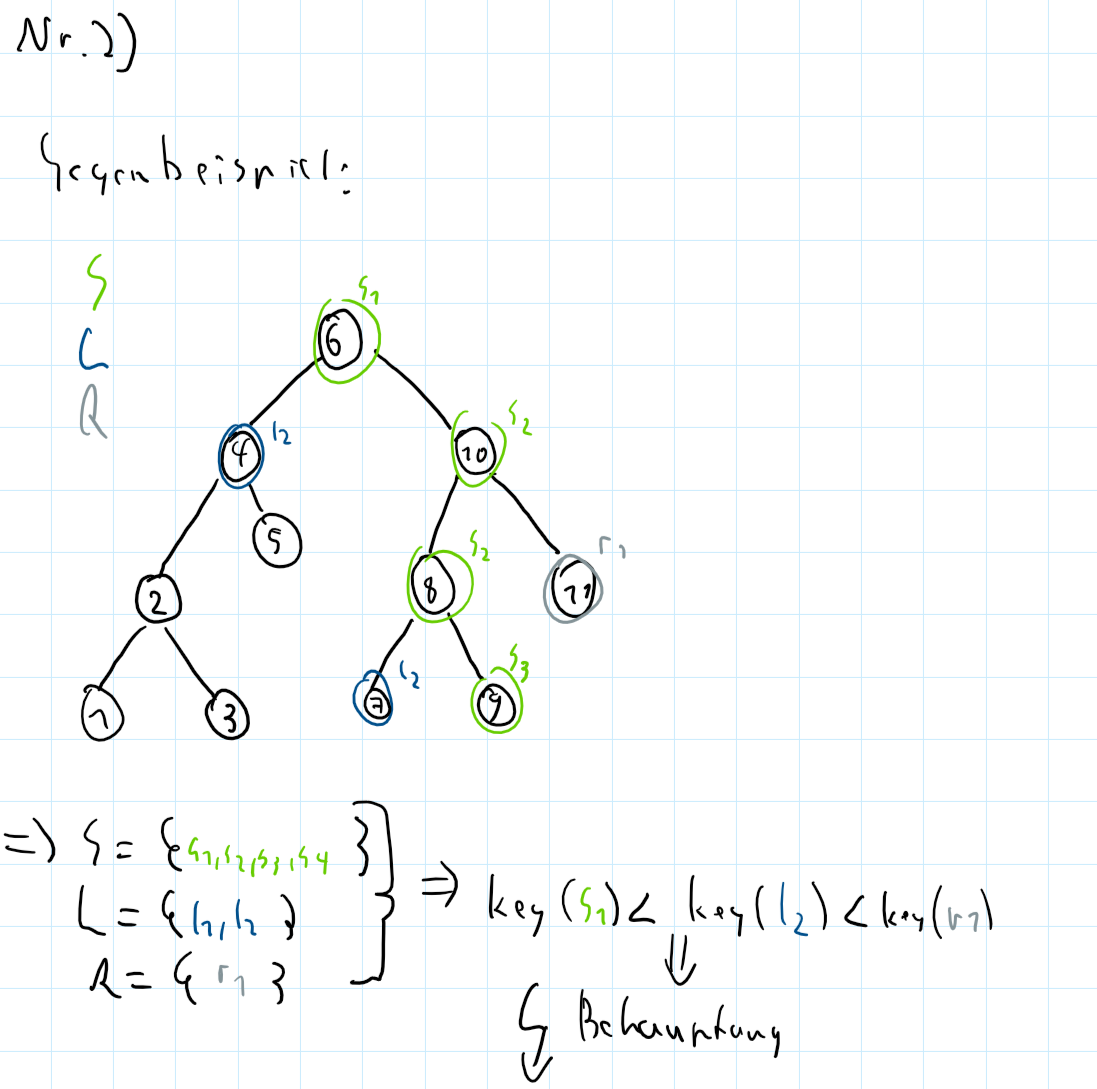
\includegraphics[width=\textwidth]{2022-05-28-Blatt-7-DuA 7_2.JPG}
\end{aufgabe}

% Aufgabe 3

\begin{aufgabe}
  \begin{teilaufgabe}
    Es wird Inorder-Tree-Walk(x), mit Vertauschung von lc[x] mit rc[x] und statt einer Ausgabe wird list-insert (L,x) aufgerufen. \\
    Dadurch wird eine absteigende Sortierung der Schlüssel an list-insert übergeben wodurch eine aufsteigend sortierte Link-list entsteht. Zum Beginn des Algorithmus wird x auf root[T] gesetzt und die Liste L ist leer.\\
    \begin{algorithm}[H]
      \caption{bin-Search-to-linked-list(T,L,x)}
      \begin{algorithmic}[1]
        \If{$x \neq nil$}
        \State bin-Search-to-linked-list(T,L,rc[x])
        \State List-Insert(L,x)
        \State bin-Search-to-linked-list(T,L,lc[x])
        \EndIf
      \end{algorithmic}
    \end{algorithm}
  \end{teilaufgabe}
  \begin{teilaufgabe}
    Z.z Der Algorithmus ist Korrekt $ \Longleftrightarrow$ Die Elemente in L sind aufsteigend sortiert. \\
    o.B.d.A Ist dies der Fall, falls List-insert die Adressen der Elemente des Baumes und die Elemente in einer absteigenden sortierten Reihenfolge übertragen werden. \\
    $\Rightarrow$ Es ist nur noch zu zeigen, dass die Elemente des Baumes in einer absteigenden sortierten Reihenfolge an List-Insert übertragen werden. (Das die Adressen dieser übertragen werden gilt nach Zeile 3). \\
    Beweis durch Vollständige Induktion über die Anzahl der Element eines Baumes mit Hilfe der Suchbaumeigenschaft. \\
    Sei $T_{n}$:= ein beliebiger binärer Suchbaum mit n Elementen \\
    IA: n = 0: Trivial\\
    n = 1: Trivial \\
    n = 2: Trivial  \\
    %%n = 3: \\
    %%Sei x:= das rechteste Blatt von $T_{3}$
    %%Der Algorithmus wird über: \\
    %%bin-Search-to-linked-list($T_{3}$,L,(root[$T_{3}$])) aufgerufen. \\
    %%Nun wird Zeile 2, solange rekursiv ausgeführt bis x erreicht ist. \\
    %%Dieses ist nach der binären Suchbaumeigenschaft das größte Element von $T_{3}$. \\
    %%Dieses wird nach Zeile 3 an List-Insert übertragen. \\
    %%Dannach Zeile 4 ausgefürhrt, bis der Vorgänger von x erreicht ist. \\
    %%Dieses ist nach der binären Suchbaumeigenschaft das zweit größte Element von $T_{3}$. Dieses wird übertragen. \\
    %%Dannach wird der Algorithmus solange Rekursiv ausgeführt, bis der  Vorgänger vom Vorgänger von x erreicht ist. \\
    %%Dieses ist nach der binären Suchbaumeigenschaft das dritt größte Element von $T_{3}$. Dieses wird übertragen. \\
    %% Nun wurden alle Elemente aufgerufen und der Algorithmus terminiert. \\
    IV: Es gelte: Der Algorithmus überträgt die Elemente eines Baumes $T_{n-1}$ in einer absteigenden sortierten Reihenfolge korrekt.\\
    IS: Z.Z Der Algorithmus überträgt die Elemente eines Baumes $T_{n}$ in einer absteigenden sortierten Reihenfolge korrekt. \\
    Es gilt: $T_{n}$ = $T_{n-1}$ + Einfügen ($T_{n-1}$,n) \\
    Nach IV gilt bereits das alle Elemente ohne n Korrekt ausgegeben werden. \\
    Folglich ist nur noch zu Zeigen, das n an der richtigen Stelle ausgeben wird. \\
    Dies ist, aber trivialerweise der Fall, da beim Einfügen die Suchbaumeigenschaft erhalten bleibt.\\
    $\Rightarrow$ n wird an der richtigen Stelle ausgeben.
    Nachdem Induktionsprinzip gilt, dass für einen Baum mit n elementen, die Elemente des Baumes in einer absteigenden sortierten Reihenfolge an List-Insert übertragen werden.\\
    $\Rightarrow$ Der Algorthmus ist Korrekt. \qed
  \end{teilaufgabe}
  \begin{teilaufgabe}
    bin-Search-to-linked-list ist eine abgeänderte Variante des aus der Vorlesung bekannten Algo. Inoder-Tree-Walk. \\
    Es gibt zwei Unterschiede zwischen bin-Search-to-linked-list und Inoder-Tree-Walk, welche aber keinen Einfluss auf die Laufzeit haben. \\
    Zum einen wurde rc[x] durch lc[x] ausgetauscht. (Dies hat trivialerweise keinen Einfluss auf die Laufzeit.) Zum anderen wurde return key[x] durch  List-Insert(L,x) ausgetauscht. Diese haben beide eine Laufzeit von $\mathcal{O}(1)$ (Nach Lemma 10.10)
    Folglich bleibt die Laufzeit erhalten.\\
    Da Inoder-Tree-Walk(x) nach Folie 45 eine  Laufzeit von $\theta (n)$, hat bin-Search-to-linked-list folglich auch eine Laufzeit $\theta (n)$ \\
  \end{teilaufgabe}
\end{aufgabe}

\end{document}
